% WACV 2025 Paper Template
% based on the WACV 2024 template, which is
% based on the CVPR 2023 template (https://media.icml.cc/Conferences/CVPR2023/cvpr2023-author_kit-v1_1-1.zip) with 2-track changes from the WACV 2023 template (https://github.com/wacv-pcs/WACV-2023-Author-Kit)
% based on the CVPR template provided by Ming-Ming Cheng (https://github.com/MCG-NKU/CVPR_Template)
% modified and extended by Stefan Roth (stefan.roth@NOSPAMtu-darmstadt.de)

\documentclass[10pt,twocolumn,letterpaper]{article}

%%%%%%%%% PAPER TYPE  - PLEASE UPDATE FOR FINAL VERSION
%\usepackage[review,algorithms]{wacv}% To produce the REVIEW version for the algorithms track
%\usepackage[review,applications]{wacv}% To produce the REVIEW version for the applications track
\usepackage{wacv}  % To produce the CAMERA-READY version
%\usepackage[pagenumbers]{wacv} % To force page numbers, e.g. for an arXiv version

% Include other packages here, before hyperref.
\usepackage{graphicx}
\usepackage{amsmath}
\usepackage{amssymb}
\usepackage{booktabs}
\usepackage{multirow}
\usepackage{algorithm}
\usepackage{algorithmicx} % <===========================================
\usepackage{algpseudocode} % <==========================================
\usepackage{setspace}
\usepackage{bm}
\usepackage{tikz}
\usepackage[letterpaper, left=0.68in, right=0.9in, top=1in, bottom=1.0in]{geometry}
\newcommand{\ballnumber}[1]{\tikz[baseline=(myanchor.base)] \node[circle,fill=.,inner sep=1pt] (myanchor) {\color{-.}\bfseries\footnotesize #1};}
% It is strongly recommended to use hyperref, especially for the review version.
% hyperref with option pagebackref eases the reviewers' job.
% Please disable hyperref *only* if you encounter grave issues, e.g. with the
% file validation for the camera-ready version.
%
% If you comment hyperref and then uncomment it, you should delete
% ReviewTempalte.aux before re-running LaTeX.
% (Or just hit 'q' on the first LaTeX run, let it finish, and you
%  should be clear).

\usepackage[pagebackref,breaklinks,colorlinks]{hyperref}


% Support for easy cross-referencing
\usepackage[capitalize]{cleveref}
\crefname{section}{Sec.}{Secs.}
\Crefname{section}{Section}{Sections}
\Crefname{table}{Table}{Tables}
\crefname{table}{Tab.}{Tabs.}


%%%%%%%%% PAPER ID  - PLEASE UPDATE
\def\wacvPaperID{26} % *** Enter the WACV Paper ID here
\def\confName{WACV}
\def\confYear{2026}

\usepackage[symbol]{footmisc}
\def\correspondingauthor{\footnote{Corresponding author.}}

\begin{document}

%%%%%%%%% TITLE - PLEASE UPDATE
\title{MergeSlide: Continual Model Merging and Task-to-Class Prompt-Aligned Inference for Lifelong Learning on Whole Slide Images}

\author{Doanh C. Bui$^{1,}$\textsuperscript{*}, Ba Hung Ngo$^2$, Hoai Luan Pham$^1$, Khang Nguyen$^3$, Ma\"{i} K. Nguyen$^4$, Yasuhiko Nakashima$^1$ \\
$^1$Nara Institute of Science and Technology, Japan \\
$^2$Graduate School of Data Science, Chonnam National University, South Korea \\
$^3$University of Information Technology, Viet Nam National University Ho Chi Minh City, Viet Nam \\
$^4$ETIS (UMR 8051), CY Cergy Paris University, ENSEA, CNRS, France \\
{\tt\small bui.cao\_doanh.bd2@naist.ac.jp \quad ngohung@chonnam.ac.kr \quad pham.luan@is.naist.jp} \\
{\tt\small khangnttm@uit.edu.vn \quad mai.nguyen-verger@cyu.fr \quad nakashim@is.naist.jp}
}

\maketitle

\footnotetext[1]{Corresponding author.}

\begin{abstract}

Lifelong learning on Whole Slide Images (WSIs) aims to train or fine-tune a unified model sequentially on cancer-related tasks, reducing the resources and effort required for data transfer and processing, especially given the gigabyte-scale size of WSIs.
In this paper, we introduce MergeSlide, a simple yet effective framework that treats lifelong learning as a model merging problem by leveraging a vision-language pathology foundation model. When a new task arrives, it is:
\ballnumber{1} defined with class-aware prompts,
\ballnumber{2} fine-tuned for a few epochs using an MLP-free backbone, and
\ballnumber{3} merged into a unified model using an orthogonal continual merging strategy that preserves performance and mitigates catastrophic forgetting.
For inference under the class-incremental learning (CLASS-IL) setting, where task identity is unknown, we introduce Task-to-Class Prompt-aligned (TCP) inference. Specifically, TCP first identifies the most relevant task using task-level prompts and then applies the corresponding class-aware prompts to generate predictions.
To evaluate MergeSlide, we conduct experiments on a stream of six TCGA datasets. The results show that MergeSlide outperforms both rehearsal-based continual learning and vision-language zero-shot baselines. Code and data are available at \url{https://github.com/caodoanh2001/MergeSlide}.
% Furthermore, MergeSlide demonstrates robustness to task and dataset order, whereas other methods often show significant performance variation. These findings confirm its consistency, scalability, and flexibility. 


\end{abstract}

%%%%%%%%% ABSTRACT
\vspace{-0.5cm}
%%%%%%%%% BODY TEXT
\section{Introduction}
\label{sec:intro}


Whole Slide Images (WSIs) provide a comprehensive view of tissue at the cellular level, which is essential for cancer diagnosis and prognosis using digital computational pathology tools and protocols \cite{wu2023artificial}. In recent years, multiple-instance learning (MIL) models \cite{ilse2018attention,clam,transmil,dtfd} have become the main approach for WSI-related tasks such as tumor classification and cancer subtyping. However, with the rapid adoption of WSIs and the emergence of new cancer-related tasks, developing computational pathology tools has become increasingly challenging \cite{gou2025queryable}. {Due to their gigabyte-scale size, training deep unified multi-purpose models for WSIs is time-consuming, as it often requires substantial resources for data transfer, preprocessing, feature extraction, and model storage \cite{shen2022federated}. Moreover, data privacy concerns across institutions restrict data sharing, hindering the development of multi-purpose models that leverage diverse WSIs from multiple sources.}

\begin{figure}[!http]
\centerline{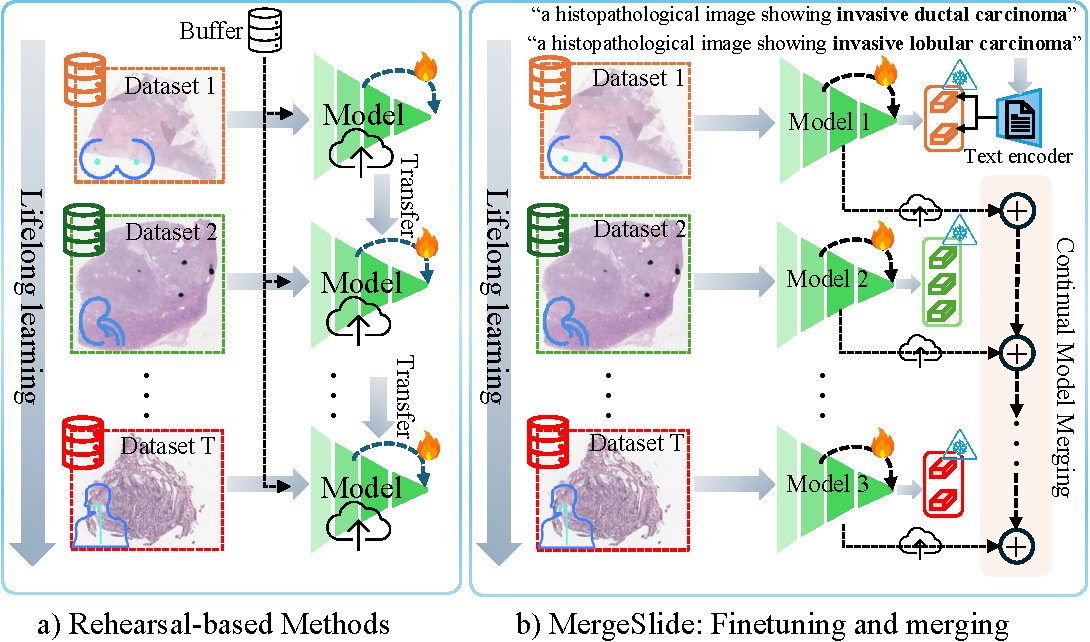
\includegraphics[width=0.49\textwidth]{thumbnail.pdf}}
\caption{\textbf{(a) Rehearsal-based methods}; \textbf{(b) Task-specific fine-tuning and merging in MergeSlide}; MergeSlide first trains an MLP-free model offline using frozen class-aware prompt embeddings. Then, the weights are merged task-by-task.}
\label{fig:thumbnail} 
\end{figure}

\begin{figure*}[http]
\centerline{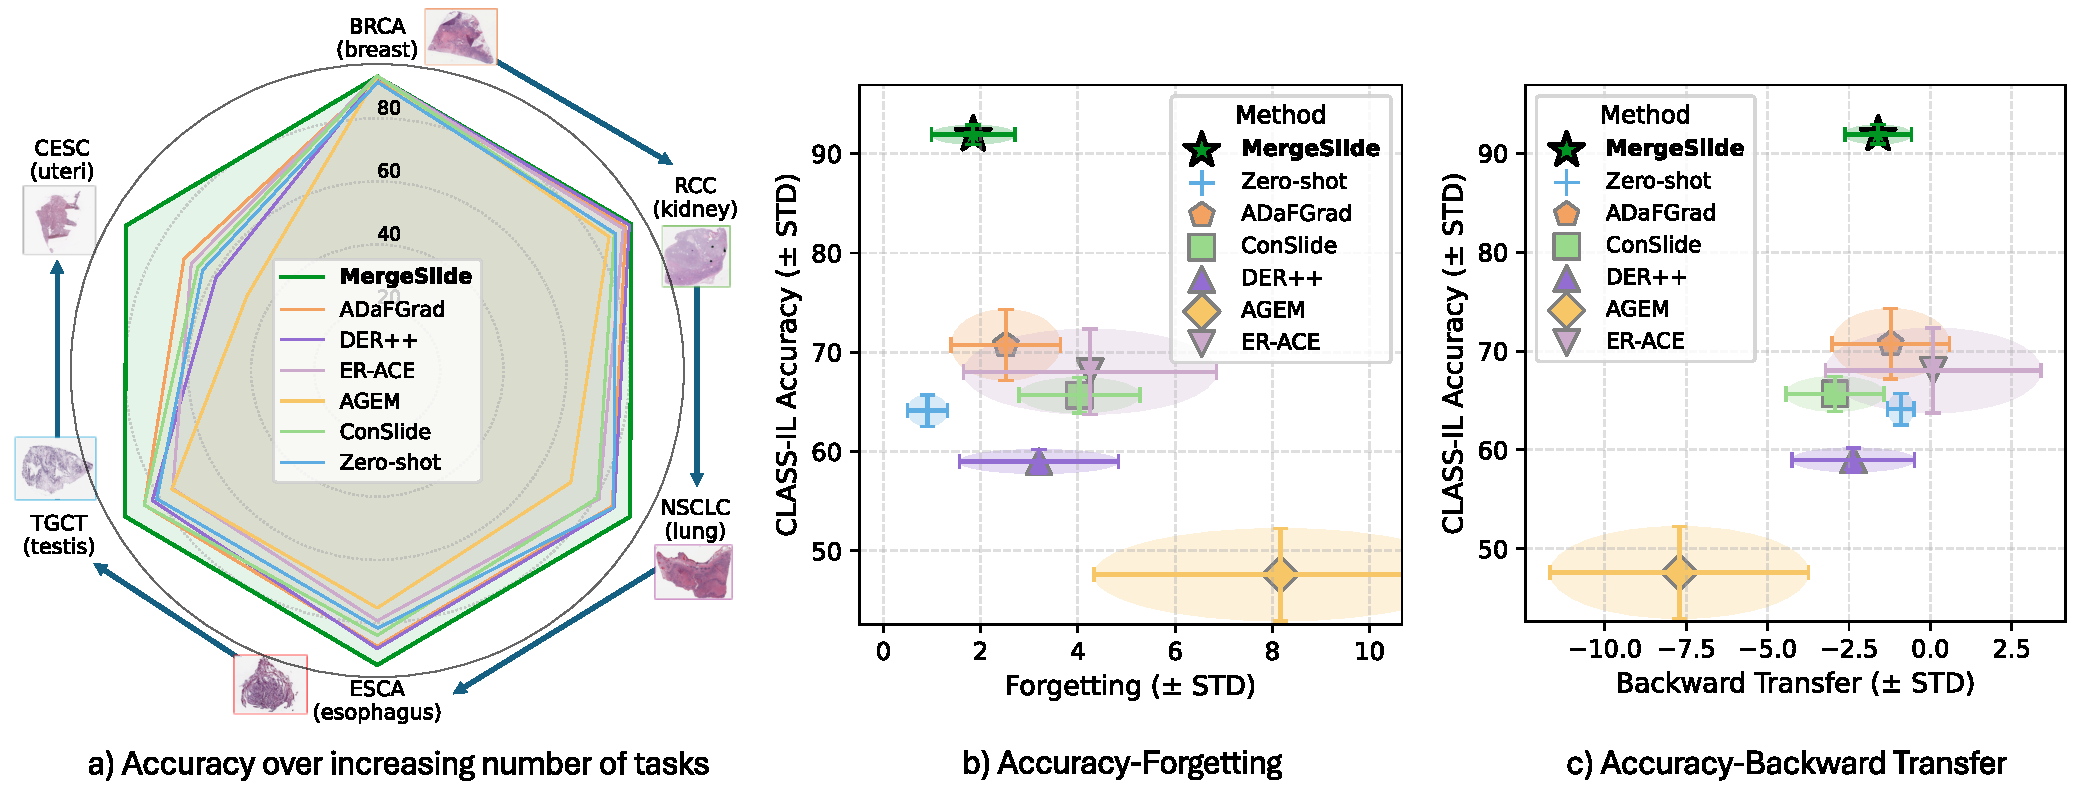
\includegraphics[width=0.85\textwidth]{radar_chart.pdf}}
\caption{\textbf{Performance comparison of MergeSlide with other continual learning methods.} (a) Accuracy as tasks accumulate. (b) Accuracy vs. Forgetting. (c) Accuracy vs. Backward Transfer, both after the final task.}
\label{fig:radarchart}
\end{figure*}

An effective solution could be to develop a single core model or tool that is continuous, adaptive, and scalable as new tasks are introduced. A naive approach might be fine-tuning a baseline model task-by-task, but this often leads to catastrophic forgetting \cite{mccloskey1989catastrophic,boschini2022transfer}, which is a phenomenon where a model trained on a new task forgets or performs poorly on previously learned tasks. To tackle this, traditional lifelong learning \cite{de2021continual} (also known as continual learning) approaches are possible \cite{huang2023conslide,gou2025queryable}. These methods are generally categorized into regularization-based and rehearsal-based techniques. Regularization-based models \cite{li2017learning,rebuffi2017icarl,kirkpatrick2017overcoming,zenke2017continual,aljundi2018memory} typically incorporate mechanisms to prevent the model from deviating too far from previous tasks when learning new ones. In contrast, rehearsal-based models \cite{agem,derpp,erace,huang2023conslide} relax this constraint by allowing the model to revisit a small buffer containing samples from previous tasks. As an early attempt to apply lifelong learning to WSIs, ConSlide \cite{huang2023conslide} introduced a breakup-and-recognize strategy to diversify buffered WSIs. Later on, with the emergence of pathology vision-language foundation models (VLMs) \cite{lu2023visual,huang2023visual,lu2024visual,ding2024multimodal} that align images with diagnostic texts, \cite{huang2024free} demonstrated that such models can effectively boost downstream WSI performance through vision-text interaction. Building on this, \cite{gou2025queryable} employed class prompts as query prototypes to enhance lifelong learning using foundation models. Nonetheless, we argue that these models have certain drawbacks:
Rehearsal-based methods often outperform others but \textit{\textcircled{\raisebox{-0.9pt}{1}} pose a risk of data leakage as well as additional memories due to the use of buffers.}
\textit{\textcircled{\raisebox{-0.9pt}{2}} The implementation of these models typically assumes that tasks have the same number of classes, {and that the maximum logits for classification must be predefined regardless of the number of incoming tasks}}, which is impractical. In practice, the number of classes should be defined flexibly by domain experts rather than constrained by the method. Finally, \textit{\textcircled{\raisebox{-0.9pt}{3}} these models are sensitive to the order of tasks}; that is, their performance is not guaranteed to remain consistent when the task order changes, as their training schemes heavily rely on interactions with previous parameters or WSIs stored in a buffer. In another line of research, model merging methods \cite{ilharco2022editing,yadav2023ties,tang2024merging} have shown that it is possible to merge parameters from individually trained models across different tasks by leveraging task vectors \cite{ilharco2022editing}, which measure the differences between each task and a well-pretrained base model that captures general knowledge. This direction is promising, as it minimizes or avoids interference with parameters across tasks during training. Nonetheless, its performance relative to continual learning models and its applicability to computational pathology remain underexplored, due to the previous lack of pathology foundation models.

In this paper, we introduce \textbf{MergeSlide}, a framework that enables efficient lifelong learning for whole slide image (WSI) analysis. An overview of MergeSlide and its comparison with rehearsal-based continual learning methods are shown in Fig.~\ref{fig:thumbnail}. Simply put, we treat lifelong learning on WSIs as a model merging process. When a new task emerges, we: \ballnumber{1} \textit{design class-aware prompts to effectively describe the target cancer subtypes and obtain their embeddings using a pathology vision--language model};  
\ballnumber{2} \textit{fine-tune for a few epochs using an MLP-free backbone with randomly sampled patches}, making it less time-consuming to develop a unified, multi-purpose WSI model. The resulting task-specific weights are then  
\ballnumber{3} \textit{incrementally merged into a unified model that retains the ability to handle all previously seen cancer-related tasks}, eliminating the need for a rehearsal buffer.  
For inference, the backbone is used solely for slide embedding, and predictions are obtained via dot-product similarity with task-level and class-aware prompt embeddings. Thanks to this design, {MergeSlide addresses the following disadvantages:  
\textit{\textcircled{\raisebox{-0.9pt}{1}} MergeSlide reduces the time required to develop a unified, multi-purpose giga-scale WSI model:} since fine-tuning is performed individually for each task and then merged into a unified model, it avoids repeatedly training the entire model from scratch when new tasks appear.
\textit{\textcircled{\raisebox{-0.9pt}{2}} MergeSlide preserves data privacy:} it does not require a rehearsal buffer, thereby avoiding potential data leakage.}
Furthermore, one might argue that with the development of pathology VLMs, zero-shot learning on WSIs \cite{mahapatra2021medical,lu2023visual,javed2024cplip} could outperform continual learning approaches simply by defining effective prompt prototypes for new tasks. However, in this study, we demonstrate that \textit{\textcircled{\raisebox{-0.9pt}{3}} MergeSlide, with just a few finetuning epochs on a pre-trained foundation pathology model, significantly outperforms the zero-shot learning approach}, while still preserving both computational efficiency and practical applicability.
Finally, since MergeSlide accumulates fine-tuned models task by task into a single unified model through merging, \textit{\textcircled{\raisebox{-0.9pt}{4}} it is asymptotically order-free}, i.e., nearly independent of task order, as performance variation across task permutations is minimal.
All of these make MergeSlide continuous, adaptive, and efficiently scalable for lifelong learning on WSI-related tasks.
We evaluate MergeSlide on six TCGA cancer subtyping tasks under two settings: class-incremental (CLASS-IL), where task identity is unknown, and task-incremental (TASK-IL), where it is provided. Results show that MergeSlide outperforms continual learning and zero-shot baselines, achieving the best balance between accuracy and forgetting (Fig.~\ref{fig:radarchart}), demonstrating its practical utility. Our study is summarized as follows:

\begin{itemize}
\item We frame lifelong learning on WSIs as a continual model merging problem, where each task is trained separately and then incrementally merged into a unified, multi-purpose model.
\item For each task, we introduce MLP-free Task-Specific Fine-Tuning, using a pre-trained slide aggregator and predefined class prompts for prediction. {This enables open-class generalization, unlike MLP-based methods that must predefine logits regardless of the number of tasks.}
\item We present {Task-to-Class Prompt-Aligned Inference (TCP)} for the CLASS-IL scenario. In this approach, a slide embedding is aligned with class- and task-level prompt embeddings to predict the cancer subtype.
\item MergeSlide outperforms both continual learning and vision-language zero-shot baselines across six TCGA datasets under CLASS-IL and TASK-IL settings.
\end{itemize}


\section{Related Works}
\label{sec:relatedwork}
\noindent\textbf{Lifelong Learning.} Lifelong learning methods can be categorized into regularization-based and rehearsal-based approaches. For example, in regularization-based methods, EWC \cite{kirkpatrick2017overcoming} constrains model updates by penalizing changes to weights deemed important for previous tasks. In contrast, rehearsal-based methods often outperform regularization-based ones. For instance, GDumb \cite{gdumb} mitigates forgetting by retraining on a balanced memory buffer. ER-ACE \cite{erace} adjusts loss weighting during replay to balance learning between old and new tasks. A-GEM \cite{agem} reduces task interference by projecting gradients to preserve knowledge from previous tasks. DER++ \cite{derpp} enhances replay via logit distillation. There is also a line of research based on orthogonal gradient projection (OGP) that attempts to update the gradient of a new task in an orthogonal direction to the subspace spanned by previous tasks, where the task subspace is constructed using Singular Value Decomposition (SVD) \cite{lin2022trgp,yang2025revisiting}. Regarding lifelong learning for computational pathology, ConSlide \cite{huang2023conslide} pioneers continual learning for WSIs by introducing a breakup-reorganize strategy to diversify buffered WSIs. ADaFGrad \cite{adafgrad} distills gradients between current and previous classification weights \cite{du2020agree}, and applies contrastive learning between WSIs and class/negative prompts.

% \textit{Though effective, these approaches introduce memory overhead and a risk of data leakage due to the buffer. Moreover, since they alter model parameters during training, performance can vary depending on the task order.}

\noindent\textbf{Model Merging Strategies.} Model merging combines weights from task-specific models into a unified model while aiming to preserve performance. It typically relies on task vectors, which are differences between task-specific and general knowledge weights \cite{ilharco2022editing}. Recent works have explored weighting strategies to merge these vectors effectively \cite{ilharco2022editing,yadav2023ties,yang2023adamerging,tang2024merging}, including Mixture-of-Experts approaches \cite{yang2023adamerging,tang2024merging} and continual merging based on task vector orthogonality \cite{tang2025merging}. This strategy suits lifelong learning on WSIs, enabling offline training, preserving data privacy, and reducing cross-institution transfer. 
% \textit{However, its effectiveness on WSIs remains untested due to previously limited pathology pretrained models, and it is still unclear whether merging strategies outperform existing continual learning methods.}

\noindent\textbf{Pathology Foundation Models.} Recent work in pathology image analysis focuses on foundation models using CNNs \cite{he2016deep} or ViTs \cite{dosovitskiy2020image}, pretrained with self-supervised methods like DINO \cite{caron2021emerging} and MoCov3 \cite{chen2021empirical}. Models such as CTransPath \cite{wang2022transformer}, UNI \cite{chen2024towards} and ProvGigaPath \cite{xu2024whole} use tile- or slide-level image data only, while multimodal models like PLIP \cite{huang2023visual} and CONCH \cite{lu2024visual} leverage large vision–text pairs at the tile level. TITAN \cite{ding2024multimodal} operates at the slide level. These models are trained with vision-language contrastive learning (e.g., iBOT \cite{zhou2021ibot}, CoCa \cite{yu2022coca}). \cite{huang2024free} has shown that that using prompt embeddings from text encoder of CONCH improves downstream WSI classification tasks.

\section{Methodology}
\label{sec:methodology}

\begin{figure*}[!h]
\centerline{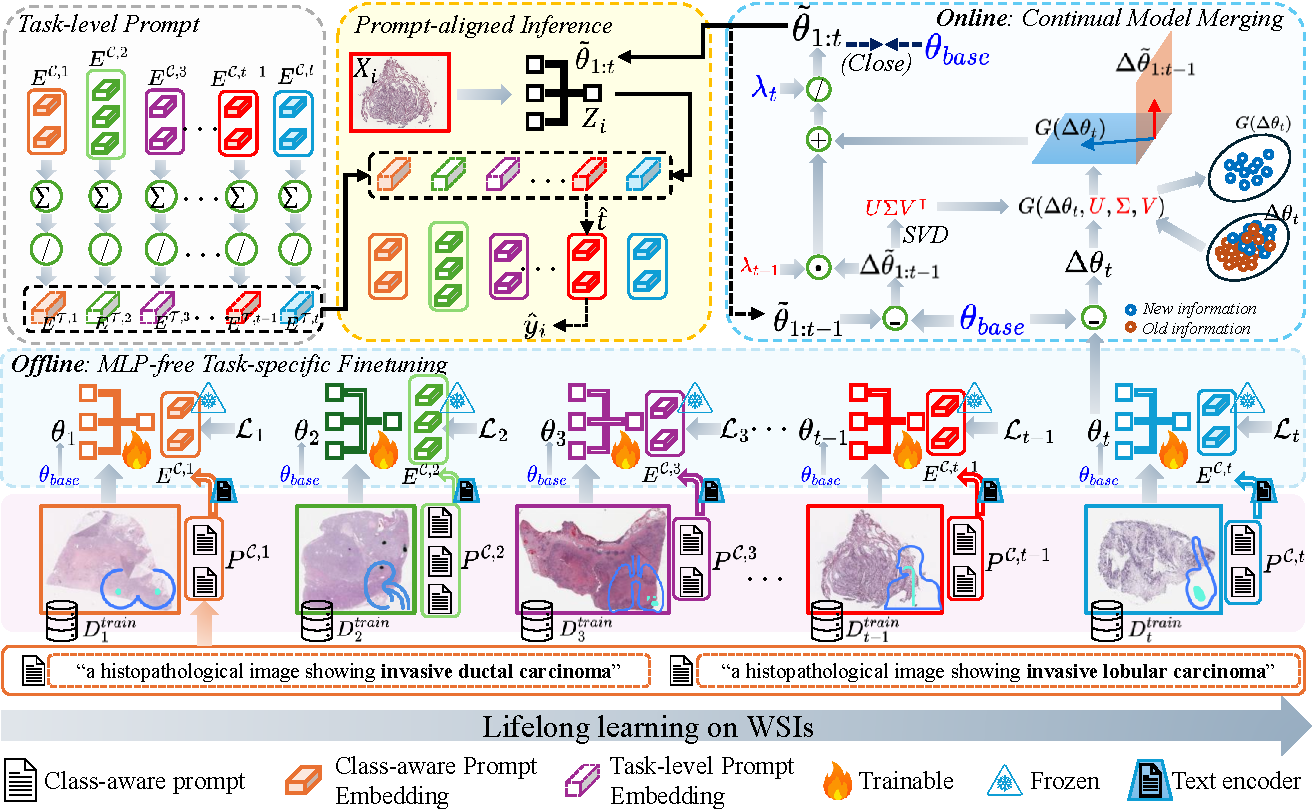
\includegraphics[width=0.9\textwidth]{main_figure.pdf}}
\caption{\textbf{Illustration of MergeSlide}. For each new task $t$, class-aware prompt embeddings $E^{\mathcal{C},t}$ are created. An \textbf{MLP-free fine-tuning step} (Sec.~\ref{sec:mlp-free}) initializes the slide aggregator $f_{\mathcal{A}}$ from base weights $\theta_{base}$, yielding task-specific weights $\theta_t$. These are then fused via \textbf{online continual model merging} (Sec.~\ref{sec:cmm}) into unified weights $\tilde{\theta}_{1:t}$ capable of handling all tasks up to $t$. Finally, \textbf{Task-to-class prompt-aligned inference} (Sec.~\ref{sec:pai}) identifies the relevant task using task-level prompts and predicts based on class-aware embeddings.}
\label{fig:mergeslide} 
\end{figure*}

\subsection{Preliminaries}

\noindent\textbf{Problem.} Given a stream of $T$ datasets $\mathcal{D} = \{D_t\}_{t=1}^T$, where each $D_t = \{D^{train}_t, D^{test}_t\}$ contains WSIs from $c_t$ cancer subtypes, the goal is to fine-tune a pre-trained slide aggregator $f_{\mathcal{A}}$ on each $D^{train}_t$ and incrementally merge the weights $\{\theta_t\}_{t=1}^{T}$ into unified weights $\tilde{\theta}_{1:T}$. The final model $f_{\mathcal{A}}(\cdot, \tilde{\theta}_{1:T})$ should generalize well across all tasks, maintaining stable performance on $\{D^{test}_t\}_{t=1}^T$. We consider two settings: (1) CLASS-IL, where task identity is unknown; and (2) TASK-IL, where it is provided at inference.

\noindent\textbf{WSI Processing.} First, for each WSI $X_i \in D_t$, it first goes through a preprocessing step. Following previous studies \cite{huang2023conslide,transmil,dtfd}, we adopt the CLAM pipeline \cite{clam}, which first segments tissue regions in the WSI using Otsu thresholding, then tiles them into patches. Each patch is processed through a frozen feature extractor; we utilize the vision encoder from TITAN \cite{ding2024multimodal}, a pathology VLM, to extract a patch embedding $v_i \in \mathbb{R}^{d_{vis}}$, where $\mathbb{R}^{d_{vis}}$ is the embedding size of each patch embedding. {It is worth noting that TITAN was chosen because it is the state-of-the-art pathology VLM, surpassing other available models such as CONCH \cite{lu2024visual} and PLIP \cite{huang2023visual}. As a direct update of CONCH, TITAN delivers stronger performance, while models like CTransPath \cite{wang2022transformer}, UNI \cite{chen2024towards} and ProvGigaPath \cite{xu2024whole} are excluded due to the absence of a well-aligned text encoder.} Finally, we obtain a bag of patch embeddings $B_i = \{v_i\}^{|B_i|}_{i=1}$.

\subsection{MergeSlide}

\noindent\textbf{Overview.} {Fig.~\ref{fig:mergeslide} illustrates MergeSlide, which consists of three stages: \textit{\textcircled{\raisebox{-0.9pt}{1}} MLP-free Fine-tuning:} For each new $t$-th task, a set of class prompts $P^{\mathcal{C},t} = \{p^{\mathcal{C},t}_i\}_{i=1}^{c_t}$ is defined, and only the slide aggregator ${f}_{\mathcal{A}}(\cdot,\theta_t)$ is fine-tuned. After training $f_{\mathcal{A}}$ on the $t$-th task, we perform \textit{\textcircled{\raisebox{-0.9pt}{2}} Model Merging:} the trained weights $\theta_t$ are merged with the accumulated weights $\tilde{\theta}_{1:t}$, integrating knowledge from all tasks so far. For inference, we introduce \textit{\textcircled{\raisebox{-0.9pt}{3}} Task-to-Class Prompt-aligned Inference:} under the CLASS-IL setting, where task identity is unknown. Given a bag of patch embeddings $B_i$ from a WSI, $B_i$ is subsampled into $B'_i$ to reduce patch count. \textit{MergeSlide} then compares the slide-level embedding $Z_i =f_{\mathcal{A}}(B'_i,\tilde{\theta}_{1:t})$ with task prompts $\mathcal{P}^\mathcal{T} = \{P^{\mathcal{T},t}\}_{t=1}^{|\mathcal{D}|}$ to predict the most relevant task $\textcolor{orange}{\hat{t}}$, and uses the corresponding class prompts $P^{\mathcal{C}, \textcolor{orange}{\hat{t}}}$ for final cancer subtype prediction. Alg.~1 in the Supplementary Material summarizes the procedure.}

\subsubsection{MLP-free Task-specific Fine-tuning}\label{sec:mlp-free} When the new $t$-th task arrives, we first initialize the weights $\theta_t$ of the slide aggregator $f_{\mathcal{A}}$ from the TITAN foundation model, denoted as $\theta_{{base}}$. A set of class prompts $P^{\mathcal{C},t} = \{p^{\mathcal{C},t}_j\}_{j=1}^{c_t}$ is then defined. The text encoder of TITAN {(which is frozen during the fine-tuning process)} is used to generate embeddings for these prompts, denoted as $E^{\mathcal{C},t} = \{e^{\mathcal{C},t}_j\}_{j=1}^{c_t}$, where $e^{\mathcal{C},t}_j \in \mathbb{R}^{1 \times d_{{text}}}$ and $d_{{text}}$ is the embedding dimension of each prompt.
To minimize training cost, given a bag of patches $B_i \in D_t$ with corresponding label $y_i$, we first apply random sampling to obtain only $K$ patch embeddings, resulting in $B'_i = \{v_j\}_{j=1}^K$ ($B'_i \in B_i$). This sampled bag $B'_i$ is then passed through $f_{\mathcal{A}}$ to obtain a slide-level embedding $Z_i$, which is subsequently compared with $E^{\mathcal{C},t}$ to compute the final logit:
\begin{equation}
Z_i = f_{\mathcal{A}}(B'_i, \theta_t), \quad \hat{p}_i = \{Z_i \cdot ({e^{\mathcal{C},t}_j})^\top| \forall e^{\mathcal{C},t}_j \in E^{\mathcal{C},t}\},
\label{eq:1}
\end{equation}
\noindent where $\hat{p}_i \in \mathbb{R}^{c_t}$ includes predicted logits for the $t$-th task. Initially, the task-specific weights are set as $\theta_t = \theta_{{base}}$. The fine-tuning process simply minimizes the cross-entropy loss for $N_e$ epochs:
\begin{equation}
\min_{\theta_t}\mathcal{L}_t (y_i, \hat{p}_i) =  \min_{\theta_t} \left(-y_i \log \hat{p}_i \right),
\label{eq:2}
\end{equation}

\noindent where $y_i \in \{0,1\}^{c_t}$ is the one-hot encoded ground truth.

\noindent\subsubsection{Orthogonal Continual Model Merging Strategy}\label{sec:cmm} From a continual model merging perspective, once the fine-tuning process for the new task $t$ is completed, its weights are merged into the accumulated weights from previous tasks. In this manner, we consider three sets of parameters: \textcircled{\raisebox{-0.9pt}{1}}: $\theta_{{base}} \in \mathbb{R}^{m\times n}$, a well-pretrained model assumed to capture general pathological knowledge; \textcircled{\raisebox{-0.9pt}{2}}: $\tilde{\theta}_{1:t-1} \in \mathbb{R}^{m\times n}$, the cumulatively merged parameters from tasks 1 to $t{-}1$; and \textcircled{\raisebox{-0.9pt}{3}}: $\theta_t \in \mathbb{R}^{m\times n}$, the newly fine-tuned parameters for the $t$-th task. \textit{The goal is to effectively merge $\theta_t$ into $\tilde{\theta}_{1:t-1}$ to obtain $\tilde{\theta}_{1:t}$, while leveraging $\theta_{{base}}$.} Following \cite{ilharco2022editing,tang2025merging}, we adopt the general update rule as follows:

\begin{equation}
\tilde{\theta}_{1:t} = \theta_{base} + \frac{\lambda_{t-1} \Delta\tilde{\theta}_{1:t-1} + G(\Delta \theta_t,\Delta\tilde{\theta}_{1:t-1})}{\lambda_t},
\label{eq:merge}
\end{equation}

\noindent where $\Delta \theta_t$ denotes the task vector \cite{ilharco2022editing}, defined as the difference between any parameter set $\theta_t$ and the general knowledge $\theta_{base}$: $\Delta \theta_t = \theta_t - \theta_{base}$. $G(\cdot)$ is a projection function designed to map the current task vector $\Delta \theta_t$ into a more efficient space. Finally, $\lambda_{t-1}$ and $\lambda_t$ are used to control the contributions of the previously merged parameters and the new task parameters, respectively. 
To derive an efficient $\tilde{\theta}_{1:t}$, we follow the principle that it should balance between $\theta_{{base}}$ and $\tilde{\theta}_{1:t-1}$: \ballnumber{a} $\tilde{\theta}_{1:t}$ must be sufficiently distant from $\tilde{\theta}_{1:t-1}$ to retain new knowledge (e.g., orthogonality \cite{lin2022trgp,yang2025revisiting}), while \ballnumber{b} ensuring that the new merged model $\tilde{\theta}_{1:t}$ does not drift too far from the general pathology knowledge $\theta_{{base}}$ provided by the foundation model. As shown in Eq.~\eqref{eq:merge}, this trade-off is governed by $\lambda_t$, $\lambda_{t-1}$, and the projection function $G(\cdot)$.

\textit{\textbf{To satisfy Condition \ballnumber{a}}}, drawing inspiration from OGP-based continual learning \cite{lin2022trgp, yang2025revisiting} and model merging techniques \cite{tang2025merging}, we aim to make $\theta_t$ orthogonal to $\tilde{\theta}_{1:t-1}$. First, we decompose $\Delta\tilde{\theta}_{1:t-1} \in \mathbb{R}^{m \times n}$ by computing the full singular value decomposition (SVD) of the previously merged model: $\Delta\tilde{\theta}_{1:t-1} = U\Sigma V^\top$, where $U \in \mathbb{R}^{m \times m}$ and $V \in \mathbb{R}^{n \times n}$ are orthogonal matrices, and $\Sigma \in \mathbb{R}^{m \times n}$ is a diagonal matrix. Since the parameter matrix $\Delta\tilde{\theta}_{1:t-1} \in \mathbb{R}^{m \times n}$ projects an $m$-dimensional vector to an $n$-dimensional one, $U$ and $V$ capture the main directions (patterns) of the input and output spaces, respectively, from previous tasks. The projection $G(\cdot)$ is then defined as:

\begin{equation}
G\left( \Delta \theta_t \right)
= U \left( \left( U^\top \Delta \theta_t V \right) \odot M \right) V^\top,
\label{eq:project}
\end{equation}

\noindent where $M$ is a zero-diagonal masking matrix that filters out the shared components between $\Delta \theta_t$ and $\Delta \tilde{\theta}_{1:t-1}$. Thanks to Eq.~\eqref{eq:project}, $\Delta \theta_t$ is projected onto the space orthogonal to $\Delta \tilde{\theta}_{1:t-1}$, i.e., $\langle G\left( \Delta \theta_t \right),\ \Delta \tilde{\theta}_{1:t-1} \rangle_F = 0$, ensuring their separability. To justify this, consider the product $G\left( \Delta \theta_t \right) \Delta \tilde{\theta}_{1:t-1}$, which simplifies to $\left( \left( U^\top \Delta \theta_t V \right) \odot M \right) \Sigma$. Since $M$ is zero on the diagonal and $\Sigma$ is diagonal, the Frobenius inner product $\langle M \odot \Sigma,\, \cdot \rangle_F = 0$. Consequently, the projection is orthogonal. \textit{In this manner, $G(\Delta\theta_t)$ extracts the novel information of the $t$-th task relative to previous tasks.} Specifically, if $\Delta\theta_t$ is well aligned with $\tilde{\theta}_{1:t}$, i.e., not novel, its projection onto the SVD basis yields dominant diagonal values. These are masked by $M$, resulting in a small $G(\Delta\theta_t)$. In contrast, if the task is novel, the off-diagonal components dominate and are preserved by $M$, producing a larger $G(\Delta\theta_t)$.

\textit{\textbf{To satisfy Condition \ballnumber{b}}}, a consistent $\|\tilde{\theta}_{1:t} - \theta_{base}\|_2$ is maintained as the number of tasks increases, and $\lambda_t$ is designed accordingly as follows:

\begin{equation}
\lambda_t = t \cdot \frac{\left\| \lambda_{t-1} \Delta \tilde{\theta}_{1:t-1} + G(\Delta \theta_t) \right\|_2}{\sum_{i=1}^{t} \left\| \theta_i \right\|_2}, \text{ where } \lambda_1 = 1.
\label{eq:lambda}
\end{equation}

\noindent To further explain how $\|\tilde{\theta}_{1:t} - \theta_{base}\|_2$ becomes consistent, let $U_t = \lambda_{t-1} \Delta\tilde{\theta}_{1:t-1} + G(\Delta \theta_t, \Delta\tilde{\theta}_{1:t-1})$. By substituting Eq. \eqref{eq:lambda} into Eq. \eqref{eq:merge} and taking the norm $\| \tilde{\theta}_{1:t} - \theta_{base} \|_2$, we obtain:

\begin{equation}
\|\tilde{\theta}_{1:t} - \theta_{base}\|_2 = \frac{1}{t} \sum_{i=1}^{t} \left\| \theta_i \right\|_2 \cdot \left\| \frac{U_t}{\|U_t\|_2} \right\|_2 = \frac{1}{t} \sum_{i=1}^{t} \left\| \theta_i \right\|_2.
\label{eq:merge}
\end{equation}

\noindent Obviously, $\frac{1}{t} \sum_{i=1}^{t} \left\| \theta_i \right\|_2 \leq \max_{i \in \{1,\dots,t\}} \left\| \theta_i \right\|_2$. Therefore, with $\lambda_t$ computed as in Eq. \eqref{eq:lambda}, the norm $\|\tilde{\theta}_{1:t} - \theta_{base}\|_2$ is upper bounded by the maximum norm of $\theta_i$. In other words, the merged weights are ensured to never drift farther from the base model than the largest single-task norm observed so far.

% \noindent where $\lambda_1 = 1$. 

% % \begin{equation}
% % U \left( \left( U^\top \Delta \theta_t V \right) \odot M \right) V^\top U\Sigma V^\top
% % \end{equation}

\noindent\subsubsection{Task-to-Class Prompt-aligned Inference}\label{sec:pai} After training on all $T$ tasks, we introduce Task-to-Class Prompt-aligned Inference to effectively leverage a pathology vision-language foundation model in the {CLASS-IL scenario}, where the target task is unknown. This process decomposes CLASS-IL scenario into two steps: \textit{\textcircled{\raisebox{-0.9pt}{1}} identifying the task most aligned with the given input WSI}, and \textit{\textcircled{\raisebox{-0.9pt}{2}} obtaining a prediction by comparing the input’s similarity to the class-aware prompts of the identified task}. To identify the most suitable task, we construct a set of $T$ task-level prompt embeddings $\mathcal{E}^\mathcal{T} = \{E^{\mathcal{T},t}\}_{t=1}^T$. For each task prompt $E^{\mathcal{T},t}$, we do not introduce a new prompt; instead, we leverage its corresponding set of class-aware embeddings $E^{\mathcal{C},t}$. Each $E^{\mathcal{C},t}$ contains a set of class-specific embeddings, which we average to obtain the task-level embedding: $E^{\mathcal{T},t} = \frac{1}{c_t} \sum E^{\mathcal{C},t}$. Then, to identify the task most aligned with a given input WSI $X_i$, we compute dot-product similarity between its slide embedding, produced by $f_{\mathcal{A}}(X_i,\tilde{\theta}_{1:T})$ and all task-level prompt embeddings in $\mathcal{E}^\mathcal{T}$. The task prediction $\textcolor{orange}{\hat{t}}$ is determined by the highest similarity score:

\begin{equation}
\textcolor{orange}{\hat{t}} = \arg \max_{t} \left\{Z_i \cdot (E^{\mathcal{T},t})^\top | \forall E^{\mathcal{T},t} \in \mathcal{E}^{\mathcal{T}}\right\}.
\end{equation}

\noindent Once the predicted target task $\textcolor{orange}{\hat{t}}$ is identified, its corresponding class-aware prompt embeddings $E^{\mathcal{C},\textcolor{orange}{\hat{t}}}$ are used to perform cancer subtyping. The prediction $\hat{p}_i$ is obtained by computing the dot-product similarity between the slide embedding $Z_i$ and the set of class-aware prompt embeddings for the $\textcolor{orange}{\hat{t}}$-th task. The predicted sub-cancer subtype is then defined by selecting the class corresponding to the maximum logit:

\begin{equation}
\hat{p}_i = \{Z_i \cdot (e^{\mathcal{C},\textcolor{orange}{\hat{t}}}_{j})^\top\vert\forall e^{\mathcal{C},\textcolor{orange}{\hat{t}}}_{j}\in E^{\mathcal{C},{\textcolor{orange}{\hat{t}}}}\}, \quad \hat{y}_i = \arg\max \hat{p}_i.
\end{equation}

\section{Experiments}
\label{sec:experiments}
\noindent\textbf{Datasets.} We use six TCGA cancer subtyping cohorts from the Genomic Data Commons (GDC) Data Portal\footnote[2]{\url{https://portal.gdc.cancer.gov/}} for training and evaluation: TCGA-BRCA (breast), TCGA-RCC (kidney), TCGA-NSCLC (lung), TCGA-ESCA (esophagus), TCGA-TGCT (testis), and TCGA-CESC (cervix uteri). Each cohort is split into 10 folds, and 10-fold cross-validation is performed to evaluate MergeSlide against other continual learning methods. The number of subtypes per cohort is reported in Tab.~\ref{tab:slide_counts}. Slide counts vary across datasets, with some cohorts having abundant data (\textit{common cohorts}) and others having limited data (\textit{rare cohorts}).

\begin{table}[ht]
\centering
\resizebox{1\linewidth}{!}{\begin{tabular}{llr}
\toprule
\textbf{Dataset} & \textbf{Subtype}  & \textbf{\# WSIs} \\
\midrule
\multirow{2}{*}{TCGA-BRCA (\textcolor{blue}{B})} & invasive ductal carcinoma (IDC) & 726  \\
   & invasive lobular carcinoma (ILC) & 149  \\
\midrule
\multirow{3}{*}{TCGA-RCC (\textcolor{blue}{R})}  & clear cell renal cell carcinoma (CC) & 498  \\
   & papillary renal cell (P)   & 289  \\
   & chromophobe renal cell carcinoma (ChRCC) & 118  \\
\midrule
\multirow{2}{*}{TCGA-NSCLC (\textcolor{blue}{N})}& squamous cell carcinoma (SCC) & 845  \\
   & adenocarcinoma (A) & 109  \\
\midrule
\multirow{2}{*}{TCGA-ESCA (\textcolor{red}{E})} & squamous cell carcinoma (SCC) & 114  \\
   & adenocarcinoma (A) & 86   \\
\midrule
\multirow{2}{*}{TCGA-TGCT (\textcolor{red}{T})} & seminoma (S) & 66   \\
   & mixed germ cell tumor (MGCT) & 29   \\
\midrule
\multirow{2}{*}{TCGA-CESC (\textcolor{red}{C})} & adenocarcinoma (A) & 270  \\
   & squamous cell carcinoma (SCC) &  49   \\
\bottomrule
\end{tabular}}
\caption{\textbf{Number of WSIs per cancer subtype for each TCGA cohort.} Abbreviations of rare cohorts are highlighted in \textcolor{red}{red}, while those of common cohorts are highlighted in {blue}.}
\label{tab:slide_counts}
\end{table}

\noindent \textbf{Metrics.} For evaluation, we use three primary accuracy metrics and two primary continual learning metrics.

\begin{table*}[]
\centering
\resizebox{1\linewidth}{!}{\begin{tabular}{l|c|lll|cc}
\toprule
\multicolumn{1}{c|}{\textbf{Method}} & \textbf{Buffer size} & \multicolumn{1}{c}{\textbf{\begin{tabular}[c]{@{}c@{}}{bACC} $\uparrow$\\ {(CLASS-IL)}\end{tabular}}} & \multicolumn{1}{c}{\textbf{\begin{tabular}[c]{@{}c@{}}{Masked bACC} $\uparrow$\\ {(TASK-IL)}\end{tabular}}} & \multicolumn{1}{c|}{\begin{tabular}[c]{@{}c@{}}\textbf{Mean ACC}$\uparrow$\\ \textbf{(CLASS-IL)}\end{tabular}} & \textbf{FGT}  $\downarrow$  & \textbf{\#BWT $\uparrow$}  \\ \midrule
Fully Supervised & \multirow{3}{*}{0 WSIs}  & {81.309 ($\pm$3.064)} & {89.688 ($\pm$1.687)} & \multicolumn{1}{c|}{--} & --  & -- \\
Naive Finetuning &  & {25.673 ($\pm$2.571)} & {86.597 ($\pm$1.933)} & 69.834 ($\pm$3.566)   & 4.649 ($\pm$2.558)  & -8.035 ($\pm$3.795) \\
Zero-shot & & {68.243 ($\pm$2.558)}$^{***}$ & {86.814 ($\pm$2.105)}$^{***}$ & 82.593 ($\pm$0.017)$^{***}$ & \textbf{0.909 ($\pm$0.406)} & -0.909 ($\pm$0.406) \\
\midrule
ER-ACE \cite{erace}  & \multirow{5}{*}{10 WSIs} & {44.354 ($\pm$4.280)} $^{***}$ & {67.407 ($\pm$5.282)} $^{***}$ & 71.663 ($\pm$3.265)$^{***}$ & \multicolumn{1}{l}{5.095 ($\pm$2.429)} & -0.320 ($\pm$1.211)  \\
AGEM \cite{agem} &  & \multicolumn{1}{l}{{42.076 ($\pm$4.287)}$^{***}$}& {80.364 ($\pm$2.206)}$^{***}$ & 74.514 ($\pm$4.016)$^{***}$ & \multicolumn{1}{l}{8.167 ($\pm$3.836)} & -7.714 ($\pm$3.978)   \\
DER++ \cite{derpp} &  & {52.033 ($\pm$4.272)} $^{***}$ & {84.735 ($\pm$2.407)}$^{***}$ & 81.786 ($\pm$1.575)$^{***}$ & \multicolumn{1}{l}{4.266 ($\pm$1.089)} & -3.627 ($\pm$1.182) \\
ConSlide \cite{huang2023conslide} &  & {62.731 ($\pm$4.488)}$^{***}$ & {87.027 ($\pm$2.553)}$^{***}$ & 81.992 ($\pm$1.055)$^{***}$ & \multicolumn{1}{l}{4.849 ($\pm$2.527)} &  \textbf{0.196 ($\pm$1.745)} \\ 
ADaFGrad \cite{adafgrad} &  & {65.267 ($\pm$2.235)}$^{***}$ & {89.458 ($\pm$2.299)}$^{***}$ & 83.651 ($\pm$1.755)$^{***}$ & \multicolumn{1}{l}{2.772 ($\pm$1.633)} &  -1.589 ($\pm$1.693) \\ \midrule
ER-ACE \cite{erace}  & \multirow{5}{*}{30 WSIs} & {58.556 ($\pm$5.654)}$^{***}$ & {75.255 ($\pm$5.161)}$^{***}$ & 81.138 ($\pm$2.464)$^{***}$ & \multicolumn{1}{l}{4.251 ($\pm$2.606)} &  \underline{0.088 ($\pm$3.317)} \\
AGEM \cite{agem} &  & {42.076 ($\pm$4.287)}$^{***}$ & {80.364 ($\pm$2.206)}$^{***}$ & 74.514 ($\pm$4.016)$^{***}$ & 8.167 ($\pm$3.836)  & -7.714 ($\pm$3.978) \\
DER++ \cite{derpp} &  & {55.560 ($\pm$2.746)}$^{***}$ & {86.863 ($\pm$2.810)}$^{***}$ & 83.580 ($\pm$1.532)$^{***}$ & 3.199 ($\pm$1.640) & -2.368 ($\pm$1.889) \\
ConSlide \cite{huang2023conslide}  &  & {64.622 ($\pm$1.755)}$^{***}$ & {88.346 ($\pm$1.977)}$^{***}$ & 82.602 ($\pm$1.201)$^{***}$ & \multicolumn{1}{l}{4.032 ($\pm$1.248)} & -2.930 ($\pm$1.506) \\
ADaFGrad \cite{adafgrad} &  & {69.034 ($\pm$3.861)}$^{***}$ & {\underline{89.704 ($\pm$2.082)}}$^{***}$ & 85.469 ($\pm$1.430)$^{***}$ & 2.517 ($\pm$1.125) & -1.217 ($\pm$1.805) \\ \midrule
\textbf{MergeSlide (ours) (naive)} & \multirow{2}{*}{0 WSIs} & {\underline{80.668 ($\pm$1.860)}} & {\textbf{92.087 ($\pm$1.740)}} & \underline{90.640 ($\pm$1.247)} & 4.941 ($\pm$1.518) & 5.384 ($\pm$1.317) \\ 
\textbf{MergeSlide (ours) \texttt{w/ TCP}} &  & {\textbf{87.929 ($\pm$2.110)}} & {\textbf{92.087 ($\pm$1.740)}} & \textbf{92.686 ($\pm$0.899)} & \underline{1.848 ($\pm$0.858)} & -1.604 ($\pm$1.024) \\
\bottomrule
\end{tabular}}
\caption{\textbf{Comparison between MergeSlide and other continual learning methods on a benchmark of six TCGA datasets in the sequence of \textcolor{blue}{B}$\rightarrow$\textcolor{blue}{R}$\rightarrow$\textcolor{blue}{N}$\rightarrow$\textcolor{red}{E}$\rightarrow$\textcolor{red}{T}$\rightarrow$\textcolor{red}{C}.} p-values between the best-performing method and the others: */**/*** indicate significance at the levels of $p < 0.05$, $p < 0.01$, and $p < 0.001$, respectively. {More results, including macro/weighted F1 and precision/recall/AUC per cancer subtype from this table, are reported in Table H.1 of the Supplementary Material}.}
\label{tab:main_results}
\end{table*}

\begin{table*}[]
\centering
\resizebox{1\linewidth}{!}{\begin{tabular}{l|c|lll|cc}
\toprule
\multicolumn{1}{c|}{\textbf{Method}} & \textbf{Buffer size} & \multicolumn{1}{c}{\textbf{\begin{tabular}[c]{@{}c@{}}{bACC} $\uparrow$\\ {(CLASS-IL)}\end{tabular}}} & \multicolumn{1}{c}{\textbf{\begin{tabular}[c]{@{}c@{}}{Masked bACC} $\uparrow$\\ {(TASK-IL)}\end{tabular}}} & \multicolumn{1}{c|}{\begin{tabular}[c]{@{}c@{}}\textbf{Mean ACC}$\uparrow$\\ \textbf{(CLASS-IL)}\end{tabular}} & \textbf{FGT}  $\downarrow$  & \textbf{\#BWT $\uparrow$}  \\ \midrule
Fully Supervised & \multirow{2}{*}{0 WSIs}  & {81.151 ($\pm$2.283)} & {90.138 ($\pm$1.854)} & 84.431 ($\pm$2.304) & --  & -- \\
Naive Finetuning &  & {24.976 ($\pm$3.330)} & {86.614 ($\pm$3.543)} & 42.565 ($\pm$1.031) & 7.561 ($\pm$4.773) & -6.982 ($\pm$4.557) \\ \midrule
DER++ \cite{derpp} & \multirow{3}{*}{30 WSIs} & {61.037 ($\pm$3.319)}$^{***}$ & {84.758 ($\pm$1.929)}$^{***}$ & 78.983 ($\pm$1.955)$^{***}$ & 6.644 ($\pm$4.062) & -5.676 ($\pm$4.490) \\
ConSlide \cite{huang2023conslide}  &  & {70.821 ($\pm$2.180)}$^{***}$ & {88.896 ($\pm$2.442)}$^{**}$ & 77.146 ($\pm$1.407)$^{***}$ & 3.117 ($\pm$1.784) & -2.521 ($\pm$1.940) \\
ADaFGrad \cite{adafgrad} &  & {77.096 ($\pm$4.474)}$^{***}$ & {\underline{90.216 ($\pm$1.677)}}$^{**}$ & 81.775 ($\pm$1.227)$^{***}$ & \underline{2.304 ($\pm$1.072)} & \underline{-0.821 ($\pm$0.918)} \\ \midrule
\textbf{MergeSlide (ours) (naive)} & \multirow{2}{*}{0 WSIs} & {\underline{80.636 ($\pm$1.865)}} & {\textbf{92.109 ($\pm$1.700)}} & \underline{88.268 ($\pm$1.459)} & 4.246 ($\pm$1.585) & -1.808 ($\pm$1.987) \\ 
\textbf{MergeSlide (ours) \texttt{w/ TCP}} &  & {\textbf{87.930 ($\pm$2.112)}} & {\textbf{92.109 ($\pm$1.700)}} & \textbf{91.009 ($\pm$1.278)} & \textbf{1.807 ($\pm$0.604)} & \textbf{0.958 ($\pm$0.868)} \\
\bottomrule
\end{tabular}}
\caption{\textbf{Comparison between MergeSlide and other continual learning methods on a benchmark of six TCGA datasets in the reversed sequence of \textcolor{red}{C}$\rightarrow$\textcolor{red}{T}$\rightarrow$\textcolor{red}{E}$\rightarrow$\textcolor{blue}{N}$\rightarrow$\textcolor{blue}{R}$\rightarrow$\textcolor{blue}{B}.} p-values between the best-performing method and the others: */**/*** indicate significance at the levels of $p < 0.05$, $p < 0.01$, and $p < 0.001$, respectively. {More results, including macro/weighted F1 and precision/recall/AUC per cancer subtype from this table, are reported in Table H.3 of the Supplementary Material.}}
\label{tab:reverse}
\end{table*}

\noindent\textbf{\textit{Accuracy metrics}} include: {1) Balanced Accuracy in the CLASS\mbox{-}IL setting (\textbf{bACC}), where the task identity is unknown to the model; 2) Balanced Accuracy in the TASK\mbox{-}IL setting (\textbf{Masked bACC}), where the model is given the task indicator $(X_i, t)$ and uses the correct $E^{\mathcal{C},t}$;} 3) \textbf{Mean ACC}: the mean of overall accuracy across a sequence of $T$ tasks. {Here, balanced accuracy is the average recall across classes}, and overall accuracy is the fraction of correct predictions over all samples in the test set. \noindent\textbf{\textit{Continual learning metrics}} include: 1) \textbf{Forgetting (FGT)}, which measures the decrease in CLASS\mbox{-}IL overall accuracy for task $t$ from its peak to its value after the final task; 2) \textbf{Backward Transfer (BWT)}, which quantifies how learning a new task affects performance on earlier tasks.

\noindent\textbf{{In/Out-of-domain Evaluation.}} {Because WSIs are acquired under different settings across institutes and sites, domain shift may occur \cite{cheng2021robust}, where a model overfitted to one site does not generalize well to another. To evaluate the stability of MergeSlide under domain shift, we design \textit{in-domain (IND)} and \textit{out-of-domain (OOD)} settings. In the \textit{in-domain} setting, training and testing slides may come from the same sites, while in the \textit{out-of-domain} setting, testing slides are drawn from different sites than those used for training. This simulates realistic scenarios where new slides from unseen sites must be tested on existing models.}

\noindent\textbf{Implemental Details.} WSIs are tiled into patches of size $256 \times 256$ at $10\times$ magnification. Patch embeddings ($v_j \in B'_i$) and prompt embeddings $e^{\mathcal{C},t}_j$ (from prompts $p^{\mathcal{C},t}_j \in P^{\mathcal{C},t}$) are extracted using TITAN's vision and text encoders, both producing 768-dimensional outputs across all methods. {Class-aware prompts used to extract embeddings are described in detail in Sec.~C of the Supplementary Material.} All experiments use the AdamW optimizer \cite{loshchilov2017decoupled} on a single RTX 8000 (48~GB) GPU. For ConSlide, we adopt the HIT backbone as in the original study, which supports both patch ($256\times256$) and region ($1024\times1024$) inputs. MergeSlide employs a Transformer aggregator $f_{\mathcal{A}}$, initialized with TITAN’s pretrained weights ($\theta_{{base}}$). All models are trained for $N_e = 10$ epochs. Rehearsal-based methods are evaluated with buffer sizes of 10 and 30 WSIs.

\noindent\textbf{Main Results (In-domain Results).} We choose the sequence \textcolor{blue}{B}$\rightarrow$\textcolor{blue}{R}$\rightarrow$\textcolor{blue}{N}$\rightarrow$\textcolor{red}{E}$\rightarrow$\textcolor{red}{T}$\rightarrow$\textcolor{red}{C} as the baseline. This sequence indicates that the model is finetuned from common to rare tasks. The main results are presented in Tab.~\ref{tab:main_results}. MergeSlide outperforms all rehearsal-based methods, achieving $\geq$18.899\% in CLASS-IL bACC, $\geq$7.217\% in Mean ACC, and $\geq$2.838\% in TASK-IL Masked bACC. Even without $\texttt{TCP}$ (considers all class-aware prompt embeddings), MergeSlide still outperforms other methods by $\geq$11.634\% and $\geq$5.171\% in terms of bACC and Mean ACC, respectively, under the CLASS-IL scenario. For forgetting (FGT), MergeSlide ranks second with –0.836\%, outperforming every trainable method (FGT $\geq$ 0.772\%) and trailing only the Zero-shot approach. Although its backward transfer (BWT) is slightly negative, it still delivers the best balance between stability and plasticity. 
% Unlike rehearsal-based methods that rely on a buffer and extensive training, 
% \textit{MergeSlide requires no buffer, similar to the zero-shot approach, and only needs minimal fine-tuning.}

\noindent\textbf{{Out-of-domain Results.}} {To assess domain shift, we evaluate all baselines and MergeSlide in the \textit{out-of-domain} setting; results are reported in Tab. \ref{tab:ood}. We additionally report the per-method difference between out-of-domain and in-domain balanced accuracy, denoted $\Delta^{\text{bACC}}_{out\text{-}in}$. Although MergeSlide shows a $-2.817\%$ bACC drop under domain shift (as do AGEM, ConSlide, and ADaFGrad), it still secures the best bACC among all methods in both CLASS-IL ($\geq$23.276\% bACC) and TASK-IL ($\geq$3.465\% bACC) settings, and it also leads in FGT ($\geq$1.304\%).}


\begin{table}[]
\resizebox{1\linewidth}{!}{{\begin{tabular}{lllcc}
\toprule
{\textbf{Method}}     & \textbf{\textbf{\begin{tabular}[c]{@{}c@{}}{bACC} $\uparrow$\\ {(CLASS-IL)}\end{tabular}}}           & \textbf{\begin{tabular}[c]{@{}c@{}}{Masked bACC} $\uparrow$\\ {(TASK-IL)}\end{tabular}}    & \textbf{{FGT}$\downarrow$}            & \textbf{{$\Delta^{\text{bACC}}_{out-in}$}$\downarrow$}             \\ \midrule
{ER-ACE} \cite{erace} & {60.808 ($\pm$4.769)}$^{***}$ & {77.125 ($\pm$4.800)}$^{***}$ & {4.447 ($\pm$2.431)}  & {+2.252}  \\
{AGEM} \cite{agem}   & {41.864 ($\pm$4.186)}$^{***}$ & {76.207 ($\pm$3.793)}$^{***}$ & {12.957 ($\pm$4.964)} & {-0.212} \\
{DER++} \cite{derpp}      & {57.951 ($\pm$3.115)}$^{***}$ & {83.469 ($\pm$2.902)}$^{***}$ & {3.994 ($\pm$1.584)}  & {+2.391}  \\
{ConSlide} \cite{huang2023conslide}   & {61.336 ($\pm$5.791)}$^{***}$ & {85.945 ($\pm$4.393)}$^{***}$ & {3.214 ($\pm$1.967)}  & {-3.286}  \\
{ADaFGrad} \cite{adafgrad} & {61.836 ($\pm$5.562)}$^{***}$ & {86.110 ($\pm$3.217)}$^{***}$ & {4.108 ($\pm$2.603)}  & {-7.198}  \\ \midrule\midrule
{MergeSlide (ours)} & \textbf{{85.112 ($\pm$1.570)}} & \textbf{{89.575 ($\pm$2.440)}} & \textbf{{1.910 ($\pm$0.089)}} & \textbf{{-2.817}} \\ \bottomrule
\end{tabular}}}
\caption{{\textbf{Comparison between MergeSlide and other continual learning methods on \textbf{out-of-domain setting} in the sequence of \textcolor{blue}{B}$\rightarrow$\textcolor{blue}{R}$\rightarrow$\textcolor{blue}{N}$\rightarrow$\textcolor{red}{E}$\rightarrow$\textcolor{red}{T}$\rightarrow$\textcolor{red}{C}.} {More results are reported in Table H.2.}} \vspace{-0.7cm}}
\label{tab:ood}
\end{table}

\section{Additional Analyses}

% \noindent In this section, we further analyze: (1) MergeSlide's effect on reversed and permuted task sequences; (2) performance as tasks accumulate; (3) MLP-free finetuning efficiency; and (4) how well subtypes are separated by $f_{\mathcal{A}}(\cdot, \tilde{\theta}_{1:T})$.

\noindent\textbf{Varying Task Orders.} First, we evaluate the rare-to-common sequence, i.e., \textcolor{red}{C}$\rightarrow$\textcolor{red}{T}$\rightarrow$\textcolor{red}{E}$\rightarrow$\textcolor{blue}{N}$\rightarrow$\textcolor{blue}{R}$\rightarrow$\textcolor{blue}{B}. High-performing methods from the main results are tested under the reversed task order, with results in Tab.~\ref{tab:reverse} showing that rehearsal-based methods are sensitive to task order. For example, DER++, ConSlide, and ADaFGrad perform better when rare tasks are presented before common ones. In contrast, \textit{MergeSlide maintains stable performance with TCP and shows only marginal degradation in bACC (-0.032\%) and Mean ACC (-1.677\%) without TCP}. We also examine alternating rare and common tasks (e.g., \textcolor{blue}{B}$\rightarrow$\textcolor{red}{C}$\rightarrow$\textcolor{blue}{R}$\rightarrow$\textcolor{red}{T}$\rightarrow$\textcolor{blue}{N}$\rightarrow$\textcolor{red}{E}), with four variations tested. As shown in Tab.~\ref{tab:sequence}, \textit{MergeSlide consistently maintains stable performance across sequences.}

\begin{table}[]
\resizebox{\linewidth}{!}{\begin{tabular}{cccc}
\toprule
\textbf{Sequence} & \textbf{{ACC}} & \textbf{{Masked ACC}} & \textbf{Mean ACC} \\ \midrule
\textcolor{blue}{B}$\rightarrow$\textcolor{red}{C}$\rightarrow$\textcolor{blue}{R}$\rightarrow$\textcolor{red}{T}$\rightarrow$\textcolor{blue}{N}$\rightarrow$\textcolor{red}{E} & 91.955 ($\pm$0.902) &  93.637 ($\pm$1.084) & 91.861 ($\pm$0.914) \\
\textcolor{red}{E}$\rightarrow$\textcolor{blue}{N}$\rightarrow$\textcolor{red}{T}$\rightarrow$\textcolor{blue}{R}$\rightarrow$\textcolor{red}{C}$\rightarrow$\textcolor{blue}{B} & 91.975 ($\pm$0.915) & 92.433 ($\pm$1.084) & 91.381 ($\pm$1.126) \\
\textcolor{red}{C}$\rightarrow$\textcolor{blue}{B}$\rightarrow$\textcolor{red}{T}$\rightarrow$\textcolor{blue}{R}$\rightarrow$\textcolor{red}{E}$\rightarrow$\textcolor{blue}{N} &  91.933 ($\pm$1.061) & 93.637 ($\pm$1.084) & 91.336 ($\pm$1.154) \\
\textcolor{blue}{N}$\rightarrow$\textcolor{red}{E}$\rightarrow$\textcolor{blue}{R}$\rightarrow$\textcolor{red}{T}$\rightarrow$\textcolor{blue}{B}$\rightarrow$\textcolor{red}{C} & 91.955 ($\pm$0.926) & 93.616 ($\pm$1.098) & 91.021 ($\pm$1.041)  \\ \midrule
$\sigma$ & 0.0149 & 0.5184 & 0.3003 \\
\bottomrule
\end{tabular}}
\caption{\textbf{Experiments on alternative task orders where rare and common tasks are placed alternately.} Column $\sigma$ indicates the standard deviation of average results across three metrics.}
\label{tab:sequence}
\end{table}

\begin{figure}[!http]
\centerline{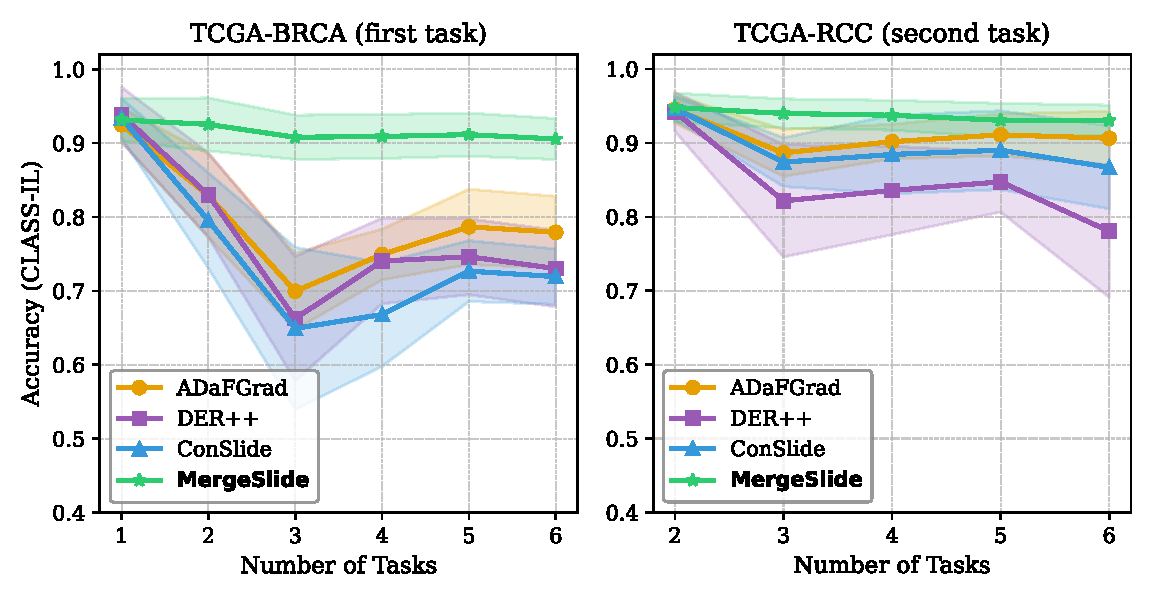
\includegraphics[width=0.49\textwidth]{forgetting.pdf}}
\caption{\textbf{Performance drop comparisons across different methods when new tasks are added on TCGA-BRCA and TCGA-RCC.} \vspace{-0.5cm}}
\label{fig:forgetting} 
\end{figure}

\noindent\textbf{Qualitative Analyses.} To take a closer look at how well tasks and cancer subtypes are recognized after training on the last task, we provide a t-SNE visualization in Fig.~\ref{fig:tsne} to show how the embeddings are clustered at both the task and class levels across the top selected methods. To further highlight the differences, we also compute the Davies–Bouldin Index (DBI) \cite{davies2009cluster}, where a lower value indicates better clustering performance. In task-level clustering, MergeSlide demonstrates superior performance on the NSCLC dataset, which is well recognized, with only two samples from ESCA and BRCA misclustered. In contrast, other methods show significant misclustering, with WSIs from the NSCLC dataset frequently mixed with those from BRCA, CESC, and RCC. In class-level clustering, IDC and ILC cancer subtypes are better separated by MergeSlide, while other methods tend to mix them together.

\begin{figure}[!http]
\centerline{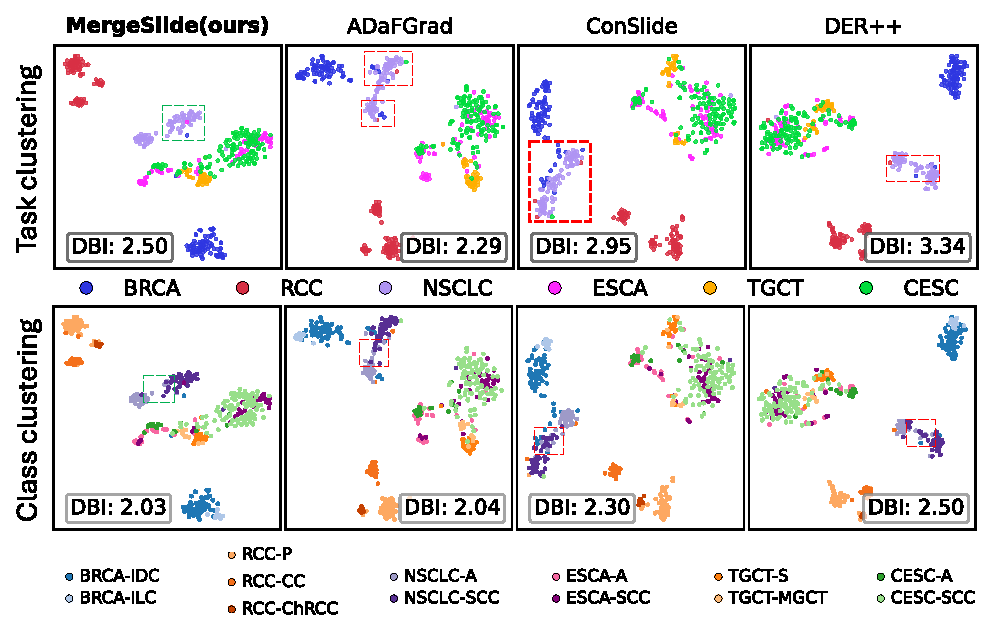
\includegraphics[width=0.49\textwidth]{tsne_vis.pdf}}
\caption{\textbf{t-SNE \cite{van2008visualizing} visualization of slide embeddings from MergeSlide and three comparative methods, organized by task and class spaces.} The dashed \textcolor{teal}{green} box highlights MergeSlide’s superior clustering, compared to the regions marked by dashed \textcolor{red}{red} boxes in other methods.}
\label{fig:tsne} 
\end{figure}

\noindent{{\textbf{Complexity Analysis of MergeSlide.} Since the slide aggregator $f_{\mathcal{A}}$ includes $L$ layers, each with weights $\theta_l \in \mathbb{R}^{m_l \times n_l}$, the overall time complexity of merging $|\mathcal{D}|$ tasks is $\mathcal{O}(|\mathcal{D}|\sum_{l=1}^{L} m_l n_l^2)$. Details are provided in Sec. I.1 of the supplementary. For empirical evaluation, Tab.~\ref{tab:complexity} reports the computational profile of MergeSlide and two strongest baselines on a single NVIDIA RTX 4090 GPU, using three metrics: average epoch time per task, GPU VRAM usage, and inference throughput. The measurements exclude WSI preprocessing (segmentation, feature extraction), as it is identical across methods. During training, MergeSlide requires more VRAM due to the orthogonal merging strategy, but its epoch time matches ConSlide and is $1.3\times$ faster than ADaFGrad. At inference, MergeSlide shows no difference with or without TCP, incurs only a slight overhead compared to ConSlide/ADaFGrad ($+0.28$s), and achieves a throughput lower by 12.07 slides/s. This trade-off remains acceptable given the substantial performance gains.}

% per_task_epoch_times
% [1.2304365634918213, 1.2196028232574463, 1.277151107788086, 0.6439673900604248, 0.38820958137512207, 0.939711332321167]
% (Pdb) throughputs
% [65.01757374063256, 71.33469875678956, 67.33737259089449, 104.04253543601524, 97.88527079984941, 136.21204256825243]

\begin{table}[]
\resizebox{1\linewidth}{!}{{
\begin{tabular}{cllccc}
\toprule
\textbf{Stage}             & \multicolumn{2}{c}{\textbf{Method}}               & \textbf{Avg. Time (s)} & \textbf{VRAM (GB)} & \textbf{Slides/s} \\ \midrule
\multirow{5}{*}{\rotatebox[origin=c]{90}{Training}}  
  & \multirow{3}{*}{MergeSlide} & Per-task FT & 74.26 & 3.38 & --  \\
  & & Merging   & 4.50 & 0.71 & --  \\ \cmidrule{3-6}
  & & Total     & 78.76 & 4.09 & --  \\ \cmidrule{2-6}
  & \multicolumn{2}{l}{ConSlide \cite{huang2023conslide}} & 78.15 & 2.90 & --  \\
  & \multicolumn{2}{l}{ADaFGrad \cite{adafgrad}}          & 104.17 & 2.70 & --  \\ \midrule
\multirow{3}{*}{\rotatebox[origin=c]{90}{Inference}} 
  & \multicolumn{2}{l}{MergeSlide (naive)} & 1.52 & 3.80 & 55.81 \\
  & \multicolumn{2}{l}{MergeSlide \texttt{\textbf{w/ TCP}}} & 1.52 & 3.89 & 55.82 \\ \cmidrule{2-6}
  & \multicolumn{2}{l}{ConSlide \cite{huang2023conslide}/ADaFGrad \cite{adafgrad}} & 1.24 & 0.87 & 67.89 \\ \bottomrule
\end{tabular}
}}
\caption{{\textbf{Computational comparison of average epoch time (s), GPU VRAM (GB), and throughput (slides/s).} MergeSlide training includes Per-task Fine-tuning (FT) and Orthogonal Model Merging. ConSlide/ADaFGrad follow the same flow during inference.}\vspace{-0.5cm}}
\label{tab:complexity}
\end{table}

\section{Conclusion}
\label{sec:conclusion}
MergeSlide enables simple yet effective lifelong learning on WSIs through class-aware prompt design, MLP-free backbone fine-tuning, and model merging. Its task-level, prompt-aligned inference leads to more accurate predictions under the CLASS-IL setting. The superior performance over both vision-language zero-shot and rehearsal-based methods demonstrates its effectiveness. Additionally, MergeSlide remains stable across different task order permutations as the number of tasks increases. 

\noindent{\textbf{Limitations \& Perspectives.} MergeSlide relies on class-aware prompts and pathology VLMs, whose textual descriptions should be carefully designed. For unseen generalization, it works naturally when new tasks arise, but handling unseen classes within existing tasks requires strategies such as class updates or out-of-distribution detection. In addition, the current orthogonal model merging uses full SVD, which may be time-consuming as tasks scale; exploring low-rank SVD is a promising direction. The performance of MergeSlide on broader tasks (e.g., cancer grades, survival bins) will also be investigated.}

{\small
\bibliographystyle{ieee_fullname}
\bibliography{egbib}
}

\end{document}
